\section{Methods}
Methodology: carefully describe the methods you use and why they are appropriate for answering your search questions. It must include
\subsection{Casual Inference}
a brief overview of causal inference, which should be written in a way such that another student in Data 100 who has never been exposed to the concept can carry out the analyses involving the datasets in your project.
\subsection{Exploratory Data Analysis}
\begin{figure}
    \centering
    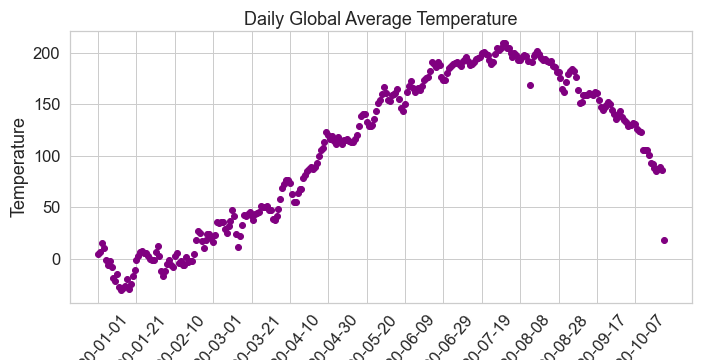
\includegraphics[width=\columnwidth]{figures/DailyAveTemp.png}
    \caption{Daily Average Temperature generated in EDA section of Analysis notebook}
    \label{fig:my_label}
\end{figure}
\subsection{Modeling}
a detailed description of how modeling is done in your project, including inference or prediction methods used, feature engineering and regularization if applicable, and cross-validation or test data as appropriate for model selection and evaluation.
